\section{Numerical Evaluation}
\label{sec:numerical-evaluation}

\subsection{Numerical Methodology and Synthetic Environments}
\label{subsec:numerical-methodology}

We evaluate architecture regret in synthetic, exogenously evolving Gaussian
environments.  The common-rate OU process in Eq.~\eqref{eq:OU_process} is
sampled exactly: for a step $\Delta$, the autoregressive coefficient is
$e^{-\Delta/T}$ and the innovation covariance is
$(1-e^{-2\Delta/T})\Sigma_S$.  For affine decisions
$x^\star=K\theta+k_0$, $K=Q^{-1}B$, information-constrained decisions are
computed by exact Gaussian conditioning.  We evaluate
$R(\mathcal A)=\tfrac12\mathbb E\|x^\star-u_{\mathcal A}^\star\|_Q^2$
both from conditional covariance and, where practical, from independently
sampled quadratic losses.  Error bars are 95\% normal confidence intervals.

Table~\ref{tab:numerical-parameters} summarizes the reference run.  Fixed
seeds are recorded with every configuration and the raw trials, processed
tables, covariance matrices, graph realizations, package versions, and
condition diagnostics are stored under \texttt{numerics/results}.  The six
experiments are regenerated by a single command documented in
\texttt{numerics/README.md}.  The largest covariance condition number in the
finite-graph experiments was $152.4$, and every constructed covariance passed
a positive-semidefinite eigenvalue check.

\begin{table}[H]
\centering
\caption{Reference numerical settings. All state variances, local stiffnesses,
and unswept coherence times are normalized to one.}
\label{tab:numerical-parameters}
\small
\begin{tabular}{llll}
\toprule
Experiment & principal sweep & size & Monte Carlo samples \\
\midrule
Temporal law & $\tau/T\in[0,3]$ & $n=8,20,32,50$ & $20{,}000$/point \\
Local--global & $\gamma/q\in[0,10]$ & $n=5,10,25,100$ & $30{,}000$/setting \\
Radius curves & $r/\ell_c\in[0,2]$ & three regimes & $50{,}000$/point \\
Radius phase & $vT/\ell_c\in[0.1,20]$ & $72\times68$ grid & covariance \\
Decision relevance & $\ell_c=0.7,2,6$ & 64-node ring & $12{,}000$/check \\
General graphs & path, ring, grid, geometric & 64 nodes & covariance \\
\bottomrule
\end{tabular}
\end{table}


\subsection{Temporal Scaling and the Local--Global Crossover}
\label{subsec:numerical-temporal-crossover}

We first tested Eq.~\eqref{eq:OU_exact_regret} on four materially different
systems: dimensions ranged from 8 to 50; $\Sigma_S$ included independent,
Toeplitz, graph-Laplacian, and geometric-graph covariances; and $Q$ and $B$
ranged from identity/dense to coupled/local operators.  Across 100 parameter
points, the Monte Carlo curves in Fig.~\ref{fig:temporal-scaling} collapse onto
$1-e^{-2\tau/T}$.  The largest absolute normalized deviation was $0.0155$ and
the root-mean-square deviation was $0.00471$; the largest discrepancy between
the empirical and direct covariance evaluations was likewise $0.0155$.
Confidence intervals are generally smaller than the plotted markers except at
the largest dimensions and delays.

\begin{figure}[t]
\centering
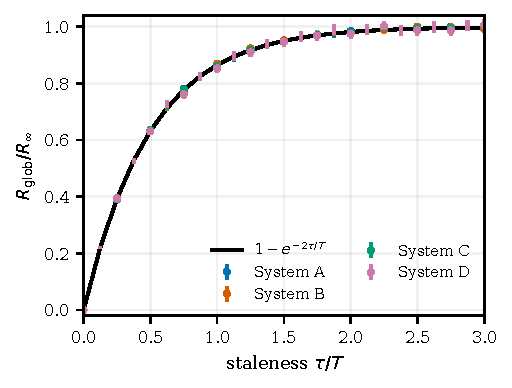
\includegraphics[width=0.82\linewidth]{numerics/figures/pdf/fig7_1_temporal_scaling.pdf}
\caption{Temporal scaling collapse. Markers are Monte Carlo estimates for four
systems with different dimensions, spatial covariances, objective matrices,
and decision operators; bars are 95\% confidence intervals. The solid curve
is the exact law $1-e^{-2\tau/T}$. Normalization by $R_\infty$ removes all
system-specific scale.}
\label{fig:temporal-scaling}
\end{figure}

We next used the shared-resource model
$Q=qI+\gamma\mathbf 1\mathbf 1^\top$, $q=1$, with independent OU components.
Figure~\ref{fig:local-global-phase} compares the empirical switch with the
exact finite-$n$ threshold in Eq.~\eqref{eq:aggregate_rho_star}.  Over 36
$(n,\gamma/q)$ settings, the mean absolute boundary error was $0.00111$ and
the maximum was $0.00557$.  Finite size matters most under strong coupling:
at $n=5$ and $\gamma/q=10$, the exact threshold is $0.109$ below the
large-system limit.  As $n$ grows, the measured boundary approaches
$\tfrac12\log(1+\gamma/q)$, confirming that stronger decision coupling
increases the amount of global staleness worth tolerating.

\begin{figure}[t]
\centering
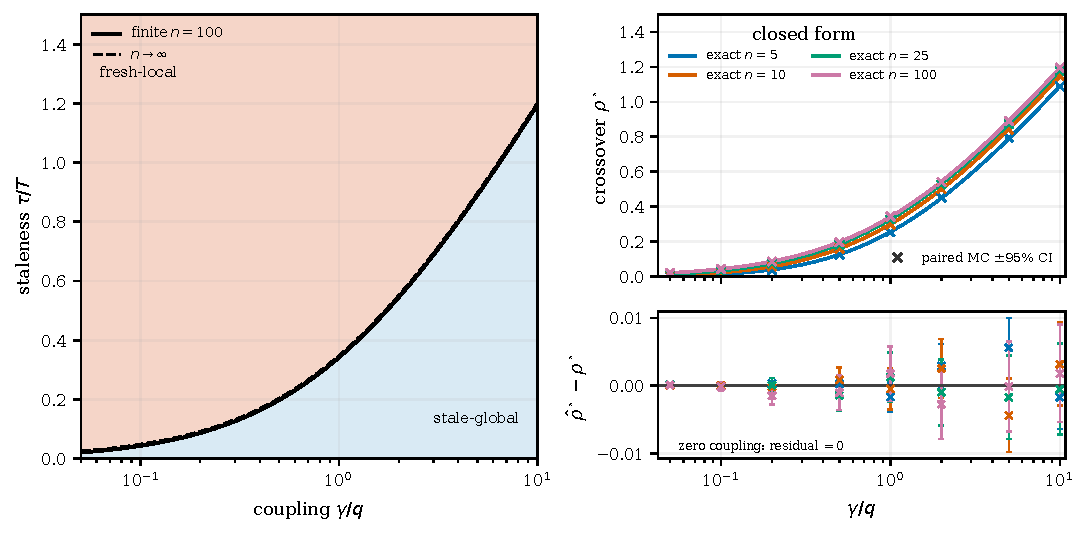
\includegraphics[width=0.98\linewidth]{numerics/figures/pdf/fig7_2_local_global_phase.pdf}
\caption{Fresh-local versus stale-global crossover. Left: winning architecture
for $n=100$; the solid finite-$n$ boundary and dashed large-$n$ boundary are
Eqs.~\eqref{eq:aggregate_rho_star} and \eqref{eq:large_n_threshold}.
Right: covariance boundaries (lines) and Monte Carlo estimates (crosses) for
four system sizes. Stronger coupling makes older global information worth
tolerating.}
\label{fig:local-global-phase}
\end{figure}

\subsection{Emergence of an Optimal Coordination Radius}
\label{subsec:numerical-radius-curves}

To expose the full tradeoff, we used
$\eta_S(r)=\eta_0e^{-2r/\ell_c}$, $\tau(r)=r/v$, and decomposed regret into
the terms $R_T(r)$ and $R_S(r)$ of Eq.~\eqref{eq:R_decomposition}.
Figure~\ref{fig:radius-regret} deliberately selects local, interior, and
boundary/global regimes on $0\le r/\ell_c\le2$.  The grid minimizers were
$0$, $0.626$, and $2.000$, respectively; the analytical capped optima were
$0$, $0.62638$, and $2.000$.  In the interior case the numerical radius error
was $3.81\times10^{-4}$ and
$|m_S(\hat r^\star)-m_T(\hat r^\star)|=4.77\times10^{-4}$, directly testing
Eq.~\eqref{eq:marginal_balance_condition}.  Independent innovation sampling
tracked the covariance curves with a worst-case absolute deviation of $0.020$
over all radii and all three regimes.

\begin{figure}[t]
\centering
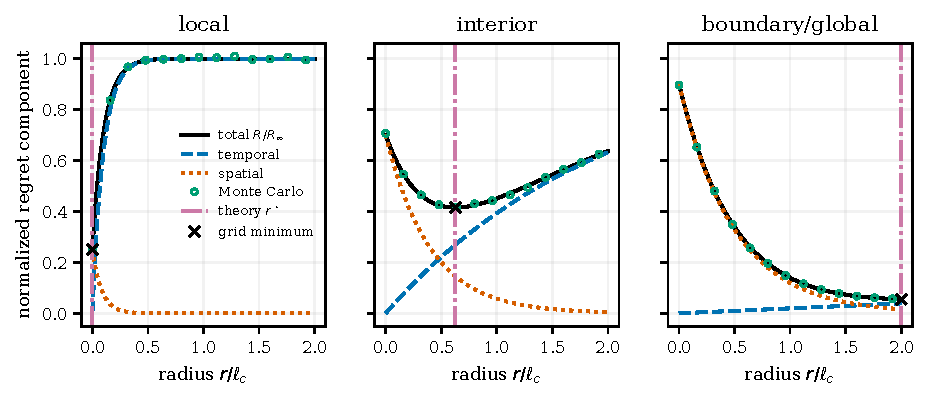
\includegraphics[width=\linewidth]{numerics/figures/pdf/fig7_3_radius_regret.pdf}
\caption{Emergence of local, interior, and boundary/global optima under
$\eta_S(r)=\eta_0e^{-2r/\ell_c}$ and $\tau(r)=r/v$. Curves show total regret
and its temporal and residual-spatial terms from Eq.~\eqref{eq:R_decomposition};
open circles are independent Monte Carlo estimates. Dash-dotted lines and
crosses mark the analytical and grid minimizers.}
\label{fig:radius-regret}
\end{figure}

\subsection{Scaling Laws and Phase Diagram}
\label{subsec:numerical-radius-phase}

We swept 4,896 points over
$vT/\ell_c\in[0.1,20]$ and $\ell_s/\ell_c\in[0.05,5]$.  At each point we
minimized Eq.~\eqref{eq:regret_composition_normalized} on a 2,501-point radius
grid independently of the closed form.  Figure~\ref{fig:radius-phase} shows
the predicted transition at $vT=2\ell_s$ and the quantitative agreement with
Eq.~\eqref{eq:canonical_dimensionless_law}: mean absolute radius error
$2.25\times10^{-4}$, maximum error $8.00\times10^{-4}$, against a maximum
grid spacing $1.60\times10^{-3}$.  Five grid points immediately adjacent to
the transition were classified as zero rather than positive because their
closed-form optima fell below one grid step; there were no discrepancies away
from that resolution band.  Separate one-dimensional numerical sweeps were
monotone in all four predicted directions: $r^\star$ increased with $T$, $v$,
and $\ell_c$, and decreased with $\ell_s$.

\begin{figure}[t]
\centering
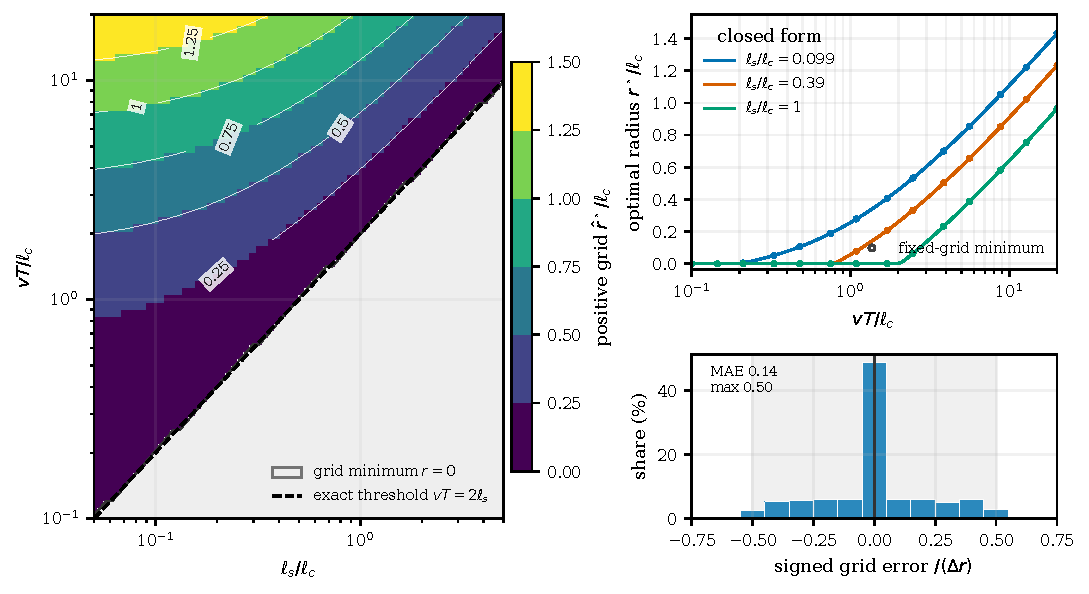
\includegraphics[width=0.98\linewidth]{numerics/figures/pdf/fig7_4_radius_phase.pdf}
\caption{Dimensionless optimal-radius law. Left: numerical
$r^\star/\ell_c$ over the $(\ell_s/\ell_c,vT/\ell_c)$ plane; the dashed line
is the predicted transition $vT=2\ell_s$. Right: grid minimizers versus the
closed form in Eq.~\eqref{eq:canonical_dimensionless_law}; the dashed line is
equality.}
\label{fig:radius-phase}
\end{figure}

\subsection{State Predictability versus Decision-Relevant Predictability}
\label{subsec:numerical-decision-relevance}

We next held a 64-node ring, its Laplacian covariance, $T=6$, and the latency
law fixed, changing only the normalized decision-sensitivity operator
$K_{ij}\propto e^{-d_G(i,j)/\ell_c}$.  Exact Gaussian conditioning gives the
curves in Fig.~\ref{fig:decision-relevance}.  Increasing $\ell_c$ from $0.7$
to $2$ to $6$ increased $\eta_S(0)$ from $0.0460$ to $0.258$ to $0.572$ and
moved the discrete optimum from 1 to 2 to 5 hops, even though the raw state
correlation was identical.  Monte Carlo conditioning checks differed from the
exact $\eta_S(r)$ by at most $3.12\times10^{-4}$.  Thus the same stochastic
environment supports substantially different architectures depending on
which spatial modes affect the desired decision.

\begin{figure}[t]
\centering
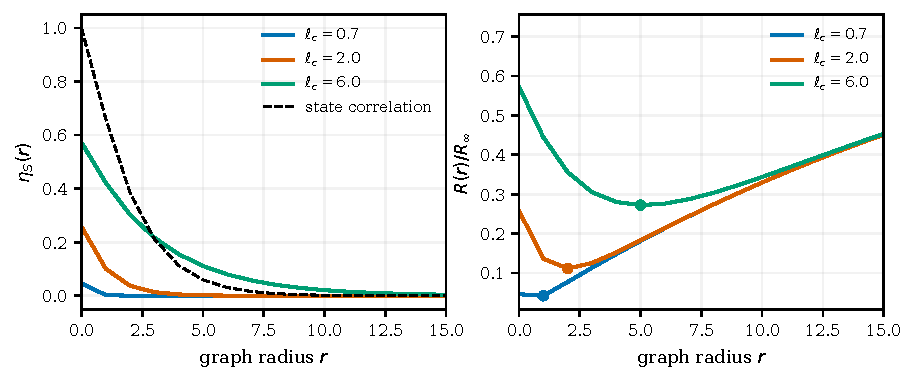
\includegraphics[width=0.94\linewidth]{numerics/figures/pdf/fig7_5_decision_relevance.pdf}
\caption{Decision relevance with the graph and state covariance held fixed.
Left: exact Gaussian spatial omission for three normalized decision operators;
the dashed raw state correlation is identical in every case. Right: composed
regret with the minimizing radius marked. Changing only the decision-relevance
range moves the optimum from 1 to 5 hops.}
\label{fig:decision-relevance}
\end{figure}

\subsection{Beyond the Canonical Line Model}
\label{subsec:numerical-general-graphs}

Finally, we considered 64-node path, ring, two-dimensional grid, and random
geometric graphs.  For each graph we formed
$\Sigma_S=(\kappa_s^2I+L_G)^{-\nu}$, normalized its marginal variance, and
computed every $\eta_S(r)$ directly from the Gaussian conditional covariance
of the desired action given the radius-$r$ neighborhood.  No exponential fit
or canonical line formula was used.  Under the common reference setting,
Fig.~\ref{fig:general-graphs} gives optima of 2, 2, 3, and 2 hops for the path,
ring, grid, and geometric graph, respectively.

Across all four graph classes, increasing $T$ from $1.5$ to $14$ changed the
optimal radius from 1 to 3 hops on the path and ring, from 1 to 4 on the grid,
and from 1 to 3 on the geometric graph.  Increasing the decision range from
$0.7$ to $6$ moved the corresponding endpoints from $(0,0,1,1)$ to
$(5,5,5,3)$.  Increasing per-hop latency weakly decreased every optimum.
Spatial smoothness was increased by decreasing $\kappa_s$ (which emphasizes
low graph frequencies after variance normalization); the optimal radii weakly
decreased, as broader measurements became more redundant.  Because radius is
discrete, these stepwise changes should be interpreted using one-hop regret
differences---the discrete analogue of marginal balance---rather than the
continuous first-order condition in Eq.~\eqref{eq:marginal_balance_condition}.

\begin{figure}[t]
\centering
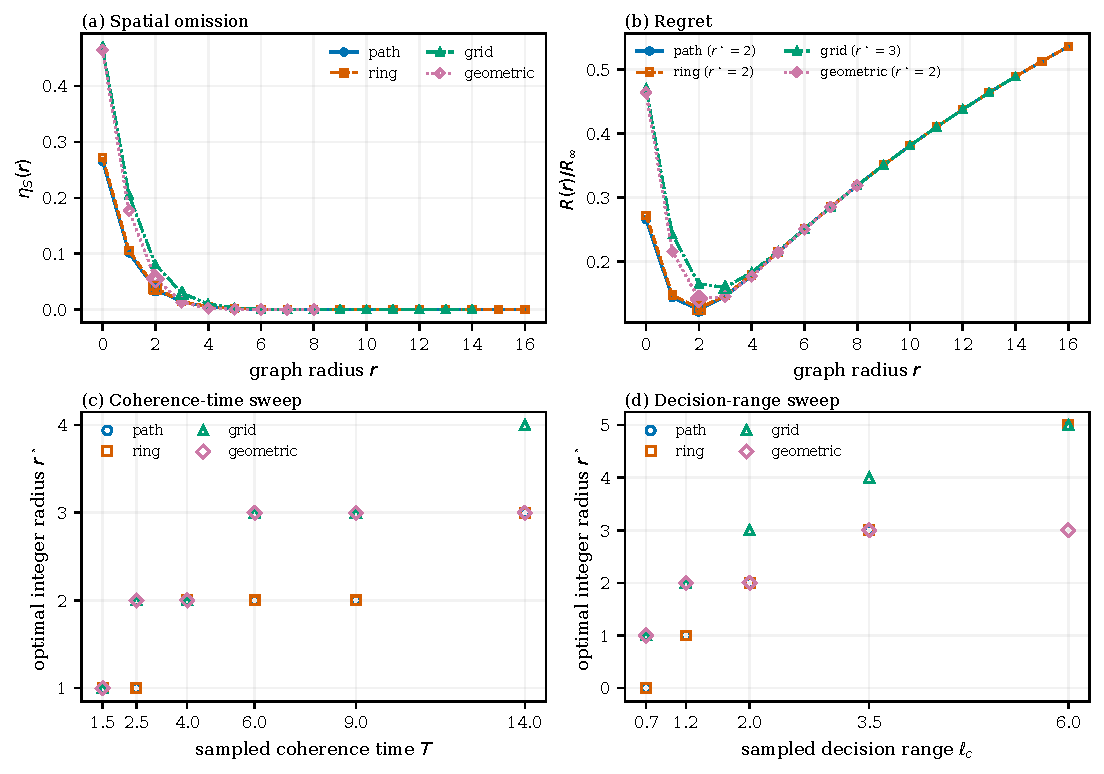
\includegraphics[width=0.94\linewidth]{numerics/figures/pdf/fig7_6_general_graphs.pdf}
\caption{Finite noncanonical graphs. Top: $\eta_S(r)$ computed from actual
Gaussian conditional covariances and the resulting regret under one common
normalized setting. Bottom: discrete optimal radius versus coherence time and
decision-relevance range. The canonical line closed form is not used; the
stepwise shifts are the discrete analogue of marginal balance.}
\label{fig:general-graphs}
\end{figure}

